\mbox{}
\thispagestyle{empty}
\newpage
\section{Drucker-Prager model of plasticity}

\subsection{Introduction}\label{sec:drucker-prager_introduction}
\indent

Drucker-Prager model of plasticity modified Mohr-Coulomb model. Unlike Mohr-Coulomb model is Drucker-Prager model yield criterion smooth and in space of the principal stresses have form of cylindrical cone. If laboratory results are in effective rather than total stress, criterion of damage become dependent on the hydrostatic and mean stress.  

\begin{figure}[h!]
	\centering	
	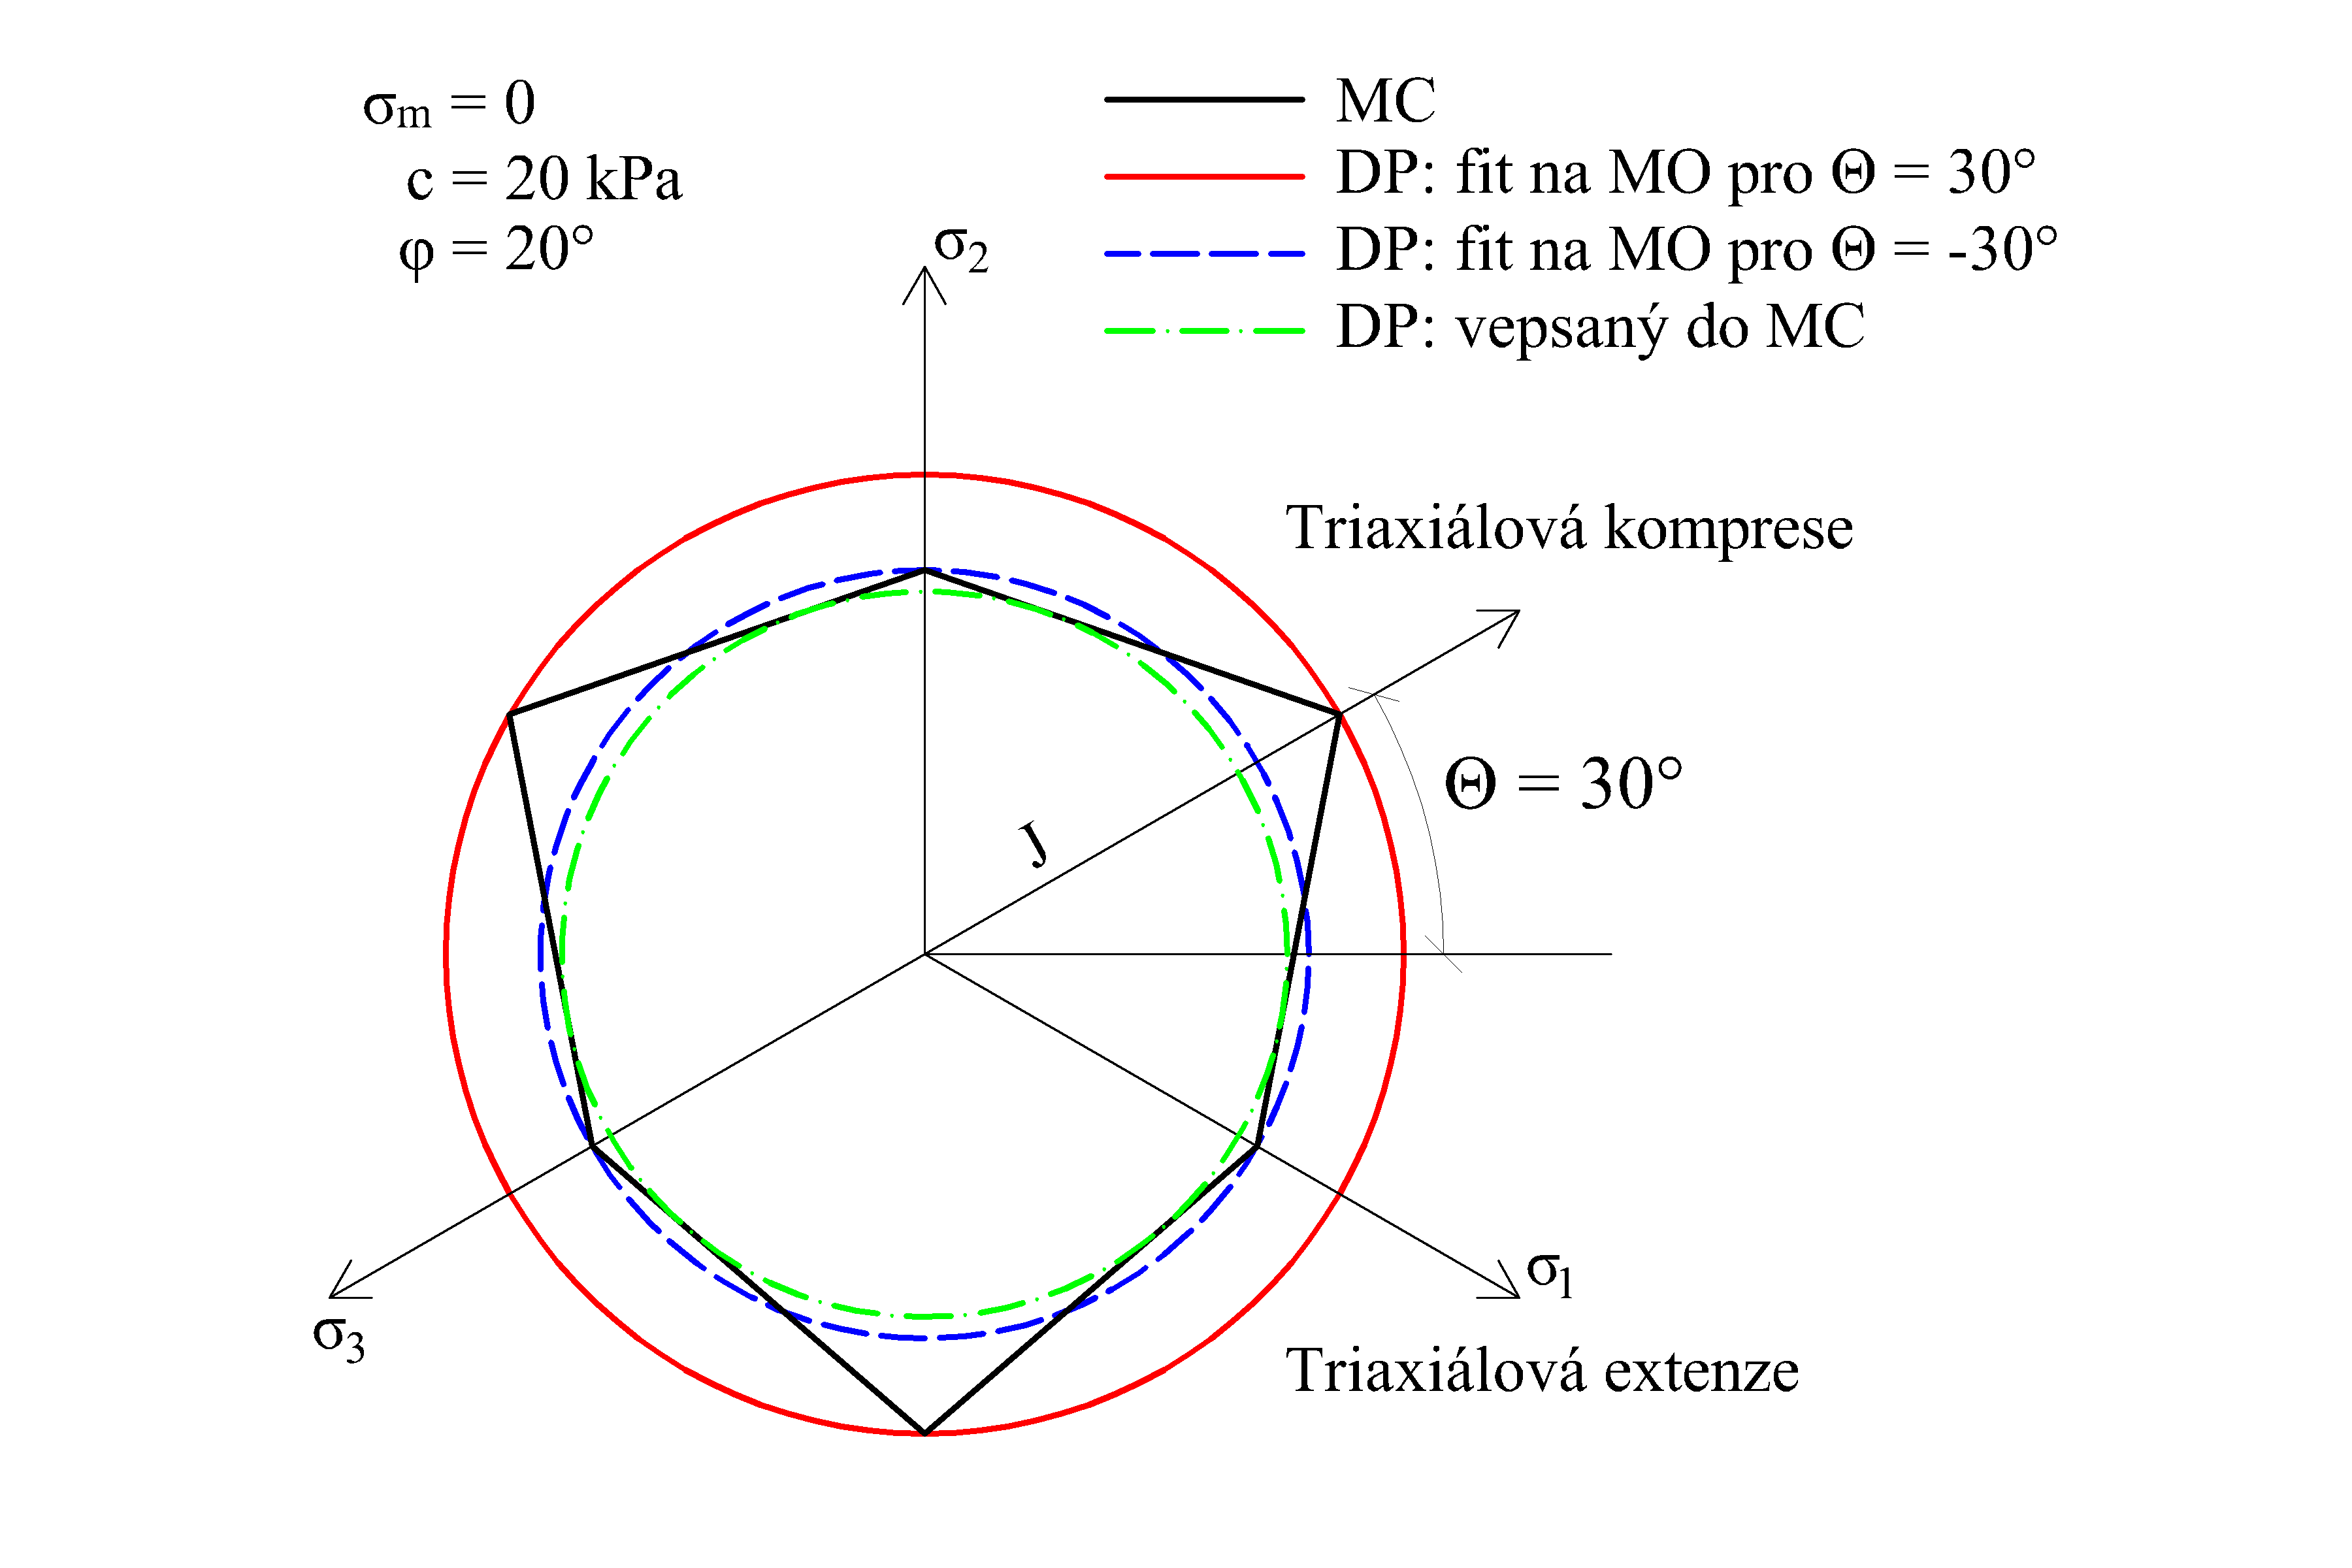
\includegraphics[width=1.1\textwidth, angle=0]{obrazky/drucker-prager.png}
	\caption[Drucker-Prager a Mohr-Coulomb model $T$]{Drucker-Prager and Mohr-Coulomb yield criterion in space of principal stresses. \label{obr:F1}}
\end{figure}

\subsection{Drucker-Prager yield criterion}\label{sec:drucker-prager_yield_criterion}
\indent

Drucker-Prager model is based on the von Mises model in that the mean stress (first invariant of stress tensor) is obtained in the yield criterion equation, which has the form  

\begin{equation}\label{eq:f_yc}
	F(\sigma) = J + (\sigma_m-c)M_{JP}(\varphi) = 0,
\end{equation}

where $J$ is second invariant of stress tensor and $M_{JP}$ is used for approximation to the Mohr-Coulomb model. Is defined as

\begin{equation}\label{eq:f_Mjp}
	M_{JP} = \dfrac{\sin(\varphi)}{cos(\theta)-\frac{\sin(\theta)\sin(\varphi)}{\sqrt{3}}},
\end{equation}

\begin{equation}\label{eq:f_theta}
	\theta = \arctan{\frac{\sin{\varphi}}{\sqrt{3}}},
\end{equation}

where $\varphi$ is tangle of internal friction. Equations \ref{eq:f_Mjp} and \ref{eq:f_theta} are used to inscribe Drucker-Prager model into Mohr-Coulomb model.
Equations (\ref{eq:f_Mjp}) a (\ref{eq:f_theta}) were taken from \cite{drucker}.

\subsection{Calculation procedure and implementation}\label{sec:drucker-prager_count}
\indent

Total elastic stress can be calculated as 
\begin{equation}\label{eq:f_sigma}
	\sigma = D \varepsilon_e,
\end{equation}
where $D$ is stiffness matrix and $\varepsilon_e$ is elastic deformation. Calculation is selected as implicit, so model is implemented with increments. Then can be equation modified as
\begin{equation}\label{eq:f_sigma1}
	\sigma^{n+1} = \sigma^n+ D \mathrm{d} \varepsilon_e.
\end{equation}
Next step in calculation is find out, if is (\ref{eq:f_yc}) satisfied, shere $\sigma_m$ a $J$ is first respective second invariant of stress tensor and are defined as

\begin{equation}\label{eq:f_J}
	J = sqrt(\frac{1}{2}\sigma^TP\sigma),
\end{equation}

\begin{equation}\label{eq:f_sigM}
	\sigma_m = m^T\sigma.
\end{equation}

If is \ref{eq:f_yc} satisfied, calculation continues with next deformation increment. If no, material become to plastic flow. Because of that is defined $\mathrm{d}\lambda$, which is coefficient of plastic flow. Dependence of $J$ and $\sigma_m$ on the $\mathrm{d}\lambda$ is taken from \cite{drucker} and have form

\begin{equation}\label{eq:f_yc_lam}
F(\sigma)= \overbrace{J-\mu\mathrm{d}\lambda}^{J^{n+1}} + (\overbrace{\sigma_m-K M_{JP}(\varphi)\mathrm{d}\lambda}^{\sigma_m^{n+1}}-c)M_{JP}=0.
\end{equation}

Coefficient of plastic flow $\mathrm{d}\lambda$ is iterating with Newton-Raphson method until is (\ref{eq:f_yc_lam}) satisfied and until are increments infinitesimal. Popsána je vztahem

\begin{equation}\label{eq:f_d_lam}
\mathrm{d}\lambda^{n+1} = \mathrm{d}\lambda^n + \frac{F^n}{F'^n}.
\end{equation}

Return to the yield of plasticity is going after normal to equation (\ref{eq:f_yc}). Normal vector is counted as \cite{drucker}

\begin{equation}\label{eq:f_n}
n = \frac{\delta F}{\delta \sigma} = \frac{1}{2J}P \sigma + M_{JP}m, 
\end{equation}

and its derivation

\begin{equation}\label{eq:f_dn}
\frac{\delta n}{\delta \sigma} = \left(\frac{3}{2}\right)^{1/2} \frac{\sigma^T P \sigma P - P \sigma \sigma^T}{(\sigma^T P \sigma)^{3/2}}.
\end{equation}
\newpage
\subsection{Return to yield of plasticity}\label{sec:drucker-prager_return}
\indent

Basic equations are

\begin{equation}\label{eq:f_r}
F(\sigma)= \overbrace{J^{res}-\mu\mathrm{d}\lambda}^{J^{n+1}} + [\overbrace{\sigma_m^{res} - K M_{PP}(\varphi^{n+1})\mathrm{d}\lambda}^{\sigma_m^{n+1}}-c^{n+1}cot(\varphi^{n+1})]M_{JP}(\varphi^{n+1})=0.
\end{equation}

\begin{equation}\label{eq:C}
C_{E_d^{pl}} = c^{n+1} - c^{i-1} - h_c^n (E_d^{pl}-(E_d^{pl})^{i-1})=0
\end{equation}

\begin{equation}\label{eq:Phi}
\varTheta_{E_d^{pl}} = \varphi^{n+1} - \varphi^{i-1} - h_{\varphi}^n (E_d^{pl}-(E_d^{pl})^{i-1})=0
\end{equation}


%
%%
%%%
%%%%následuje návrat na plochu plasticity, který se provádí pomocí metody tečen (Newton-Raphsonova metoda). Ta je definována rovnicí
%%%
%%
%

\begin{comment}
Pro binární proces $a_1 a_2 \rightarrow b_1 b_2$, kde $a \neq b$ má řídící rovnice potom tvar 

\begin{equation}\label{eq:f10}
\begin{gathered}
\dfrac{dP_n}{d t} (t) = \dfrac{G}{V} \left\langle N_{a_1} \right\rangle \left\langle N_{a_2} \right\rangle \left[ P_{n-1} (t) - P_n (t) \right] \\ - \dfrac{L}{V} \left[ n^2 P_n (t) - (n+1)^2 P_{n+1} (t) \right] ,
\end{gathered}
\end{equation}
kde $G$ je $"$kreační člen$"$ definovaný vztahem $G \equiv \left\langle \sigma _G v \right\rangle $ a $L$ je $"$anihilační člen$"$ definovaný vztahem $L \equiv \left\langle \sigma _L v \right\rangle $.


Pro hmotnosti platí 

\begin{equation}\label{eq:f12}
	m_{\pi^-} = 139.570 ~\mathrm{MeV},
\end{equation}
\begin{equation}\label{eq:f14}
	m_{\pi^0} = 134.977 ~\mathrm{MeV},
\end{equation}
\begin{equation}\label{eq:f13}
	m_n = 939.565 ~\mathrm{MeV},
\end{equation}
\begin{equation}\label{eq:f15}
	m_p = 938.272 ~\mathrm{MeV},
\end{equation}
\begin{equation}\label{eq:f16}
	d_{\pi^-} = 0,
\end{equation}
\begin{equation}\label{eq:f18}
	d_{\pi^0} = 0,
\end{equation}
\begin{equation}\label{eq:f17}
	d_{n} = 2,
\end{equation}
\begin{equation}\label{eq:f19}
	d_{p} = 2 .
\end{equation}


\begin{equation}\label{eq:f20}
\sigma (\pi^+ p \rightarrow \Delta ^{++}) = \dfrac{326,5}{1 + 4\left( \dfrac{\sqrt{s} - 1,215}{0,110} \right) ^2 } \dfrac{q^3}{q^3 + (0,18)^3},
\end{equation}

kde  

\begin{equation}\label{eq:f21}
q (cm-hybnost) = \left[ \dfrac{(s - (m_{\pi} + m_p) ^2) (s - (m_{\pi} - m_p) ^2)}{4s} \right] ^{1/2} = \dfrac{m_p}{\sqrt{s}}p_{lab}.
\end{equation}

Hodnoty hmotností a spinů byly převzány z \cite{particle}.

Zároveň platí 

\begin{equation}\label{eq:f22}
\begin{gathered}
\sigma (\pi^+ p \rightarrow \Delta ^{++}) = \dfrac{3}{2} \sigma (\pi ^0 p \rightarrow \Delta^+) = 3 \sigma (\pi^- p \rightarrow \Delta^0)  \\ = \dfrac{3}{2} \sigma (\pi^0 n \rightarrow \Delta^0) = 3 \sigma (\pi ^+ n \rightarrow \Delta^+).
\end{gathered}
\end{equation}

Dále platí pro rozpadové šířky

\begin{equation}\label{eq:f23}
\dfrac{\Gamma(\Delta^+ \rightarrow \pi^+ n)}{\Gamma (\Delta ^+ \rightarrow \pi^0 n)} = \dfrac{\Gamma (\Delta^0 \rightarrow \pi ^- p)}{\Gamma (\Delta ^0 \rightarrow \pi^0 n)} = \dfrac{1}{2}.
\end{equation}

Tedy já budu potřebovat tyto dva účinné průřezy

\begin{equation}\label{eq:f24}
\sigma (\pi^- p \rightarrow \Delta^0) = \dfrac{1}{3} \sigma (\pi^+ p \rightarrow \Delta ^{++})
\end{equation}
a
\begin{equation}\label{eq:f25}
\sigma (\pi ^0 n \rightarrow \Delta ^0) = \dfrac{2}{3} \sigma (\pi^+ p \rightarrow \Delta ^{++}).
\end{equation}

\subsection{Clebsch-Gordanovy koeficienty}\label{sec:clebsch}

Izospin a jeho projekce pro jednotlivé částice

\begin{equation}\label{eq:f26}
\Delta ^0  = \left| 3/2, -1/2 \right\rangle ,
\end{equation}

\begin{equation}\label{eq:f27}
p = \left| 1/2, 1/2 \right\rangle ,
\end{equation}

\begin{equation}\label{eq:28}
n = \left| 1/2, -1/2 \right\rangle ,
\end{equation}

\begin{equation}\label{eq:29}
\pi ^0  = \left| 1, 0 \right\rangle ,
\end{equation}

\begin{equation}\label{eq:30}
\pi ^-  = \left| 1, -1 \right\rangle .
\end{equation}

Takže pro reakci $ \Delta^0 \rightarrow n + \pi^0 $ platí

\begin{equation}\label{eq:31}
\begin{gathered}
PS: \left| 1, 0 \right\rangle \left| 1/2, -1/2\right\rangle =  
\begin{bmatrix}
1       & 1/2 & 1/2 \\
0       & -1/2 & -1/2
\end{bmatrix}
\left| 1/2, -1/2 \right\rangle + 
\begin{bmatrix}
1       & 1/2 & 3/2 \\
0      & -1/2 & -1/2 
\end{bmatrix}
\left| 3/2, -1/2 \right\rangle \\ = \sqrt{\dfrac{1}{3}} \left| 1/2, -1/2 \right\rangle + \sqrt{ \dfrac{2}{3} } \left| 3/2, -1/2 \right\rangle
\end{gathered}
\end{equation}
a
\begin{equation}
LS: \left| 3/2, -1/2 \right\rangle.
\end{equation}

Pro pravděpodobnost výskytu procesu $\Delta^0 \rightarrow n + \pi^0 $ pak platí 

\begin{equation}\label{eq:32}
\left| \left\langle \Delta^0 |  n + \pi^0 \right\rangle \right|  ^2 = \left| \sqrt{\dfrac{2}{3}} \left\langle 3/2, -1/2 | 3/2, -1/2 \right\rangle \right| ^2 = \dfrac{2}{3}.
\end{equation}

Z rovnice (\ref{eq:32}) vyplývá, že účinný průřez (\ref{eq:f24}) pro reakci $p + \pi^- \rightarrow n + \pi ^0$ přenásobíme ještě koeficientem $2/3$.

Pro reakci $ \Delta^0 \rightarrow p + \pi^- $ platí

\begin{equation}\label{eq:33}
\begin{gathered}
PS: \left| 1/2, 1/2 \right\rangle \left| 1, -1 \right\rangle =  
\begin{bmatrix}
1/2      & 1 & 1/2 \\
1/2       & -1 & -1/2
\end{bmatrix}
\left| 1/2, -1/2 \right\rangle + 
\begin{bmatrix}
1/2       & 1 & 3/2 \\
1/2     & -1 & -1/2 
\end{bmatrix}
\left| 3/2, -1/2 \right\rangle \\ = - \sqrt{ \dfrac{2}{3}} \left| 1/2, -1/2 \right\rangle + \sqrt{ \dfrac{1}{3} } \left| 3/2, -1/2 \right\rangle
\end{gathered}
\end{equation}
a
\begin{equation}
LS: \left| 3/2, -1/2 \right\rangle.
\end{equation}	

Pro pravděpodobnost výskytu procesu $ \Delta^0 \rightarrow p + \pi^- $ pak platí 

\begin{equation}\label{eq:34}
\left| \left\langle \Delta^0 |  p + \pi^- \right\rangle \right|  ^2 = \left| \sqrt{\dfrac{1}{3}} \left\langle 3/2, -1/2 | 3/2, -1/2 \right\rangle \right| ^2 = \dfrac{1}{3}.
\end{equation}

Z rovnice (\ref{eq:34}) vyplývá, že účinný průřez (\ref{eq:f25}) pro reakci $n + \pi^0 \rightarrow p + \pi ^-$ přenásobíme ještě koeficientem $1/3$.

Účinné průřezy pro reakci $p + \pi^- \rightarrow \Delta ^0 \rightarrow n + \pi ^0$ mají nakonec následující tvar


\begin{equation}\label{eq:f35}
\sigma (\pi^- p \rightarrow \Delta^0) = \dfrac{1}{3} \cdot \dfrac{2}{3} \sigma (\pi^+ p \rightarrow \Delta ^{++}) = \dfrac{2}{9} \sigma (\pi^+ p \rightarrow \Delta ^{++})
\end{equation}
a
\begin{equation}\label{eq:f36}
\sigma (\pi ^0 n \rightarrow \Delta ^0) = \dfrac{2}{3} \cdot \dfrac{1}{3} \sigma (\pi^+ p \rightarrow \Delta ^{++}) = \dfrac{2}{9} \sigma (\pi^+ p \rightarrow \Delta ^{++}).
\end{equation}


Objem reakce uvažujeme $V = 125 ~\mathrm{fm^3}$.

\subsection{Chemické složení a reakce}\label{sec:chemie}
\indent

Pro potřeby průměrování přes relativní rychlosti budeme předpokládat, že jsou hybnosti rozděleny podle Boltzmannova rozdělení 

\begin{equation}\label{eq:f1}
n_i (p) \propto exp \left( - \dfrac{\sqrt{m_{i} ^{2} + p^2}}{T} \right),
\end{equation} 
kde $p$ je hybnost, $m_i$ je hmotnost částice $i$ a $T$ je teplota.

Tím vytvoříme předpoklad tepelné rovnováhy, ale chemicky budeme systém považovat v nerovnovážném stavu.

Relativní rychlost je dána vztahem 

\begin{equation}\label{eq:f2}
v_{ij} = \left[ (p_i p_j)^2 - m_i ^2 m_j ^2 \right] ^{1/2} / E_i E_j,
\end{equation}
kde $E_i$ a $E_j$ jsou energie dvou částic.

Střední hodnota součinu účinného průřezu $\sigma _{ij} ^X$ a relativní rychlosti $v_{ij}$ je definována jako

\begin{equation}\label{eq:f3}
\left\langle \sigma _{ij} ^X v_{ij} \right\rangle = \int d^3 p_i \int d^3 p_j n_i (p_i) n_j (p_j) \sigma _{ij} ^X v_{ij} ,
\end{equation}
kde $n_k (p_k)$ jsou rozdělení hybnosti částic.

Po vyintegrování rovnice (\ref{eq:f3}) získáme požadovaný vztah pro střední hodnotu součinu účinného průřezu a relativní rychlosti ve tvaru 

\begin{equation}\label{eq:f4}
\left\langle v_{ij} \sigma_{ij} ^{X} \right\rangle  = \dfrac{\int _{\sqrt{s_0}} ^{\infty} dx \sigma_{ij} ^{X} (x) K_1 (\dfrac{x}{T}) \left[ x^2 - (m_i + m_j)^2 \right] \left[ x^2 - (m_i - m_j)^2 \right] }{4 m_{i} ^{2} m_{j} ^{2} T K_2 (m_i /T) K_2 (m_j /T)},  
\end{equation}
kde $K_i$ jsou modifikované Besselovy funkce definované vztahy 

\begin{equation}\label{eq:f5}
K_1 (z) = \int _{0} ^{\infty} e ^{- z \cosh t} \cosh (t) dt,
\end{equation}

\begin{equation}\label{eq:f6}
K_2 (z) = \int _{0} ^{\infty} e ^{- z \cosh t} \cosh (2t) dt,
\end{equation}
kde $z = x/T$.

Dále  
\begin{equation}\label{eq:f7}
\sqrt{s_0} = max(m_i + m_j, \Sigma_{final} m_a)
\end{equation}
je prahová energie reakce.

Vztahy v kapitole \ref{sec:chemie} byly převzaty z \cite{ko} a \cite{tomasik}.

Prahovou energii reakce získáme z rovnice (\ref{eq:f7})
\begin{equation}\label{eq:f37}
\begin{gathered}
\sqrt{s_0} = max (m_{\pi^-} + m_p, m_{\pi ^0} + m_{n}) \\ = max(1077.8 ~\mathrm{MeV}, 1074.5 ~\mathrm{MeV}) \simeq 1.0778 ~\mathrm{GeV}.
\end{gathered}
\end{equation}

\newpage
\subsubsection{Konstantní teplota}\label{sec:konst_teplota}
\indent

Nejprve ukážeme, jak vypadají faktoriální momenty pro řídící rovnici závislou na konstantní teplotě $T$ předělené svou rovnovážnou hodnotou, abychom mohli posoudit, jak rychle termalizují.

 Pro numerické výpočty byly použity binomické počáteční podmínky s $N_0 = 0.0005$.
 
 \begin{figure}[h!]
 	\centering	
 	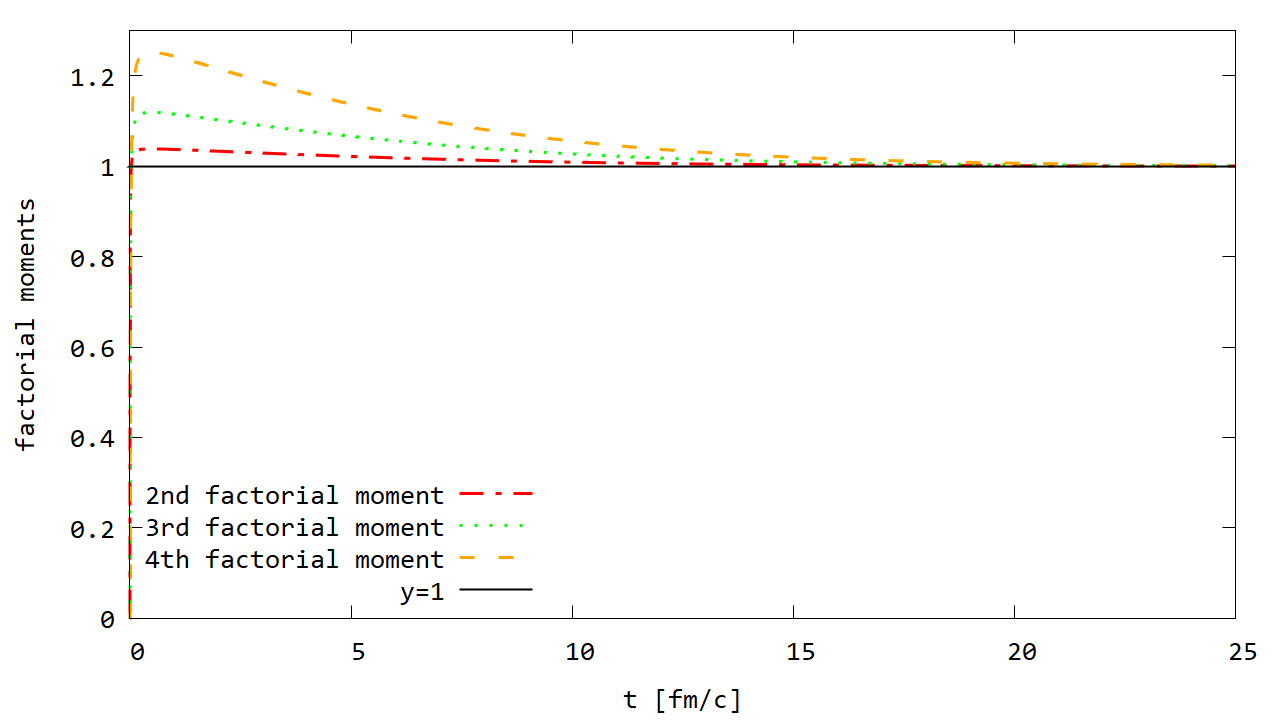
\includegraphics[width=1\textwidth, angle=0]{obrazky/fact_mom_T_165.png}
 	\caption[4. faktoriální moment pro různé teploty $T$]{Faktoriální momenty předělené svými rovnovážnými hodnotami pro teplotu $T = 165 ~\mathrm{MeV}$ pro 15 protonů a 10 pionů. \label{obr:F1}}
 \end{figure}
 
  \begin{figure}[h!]
  	\centering	
  	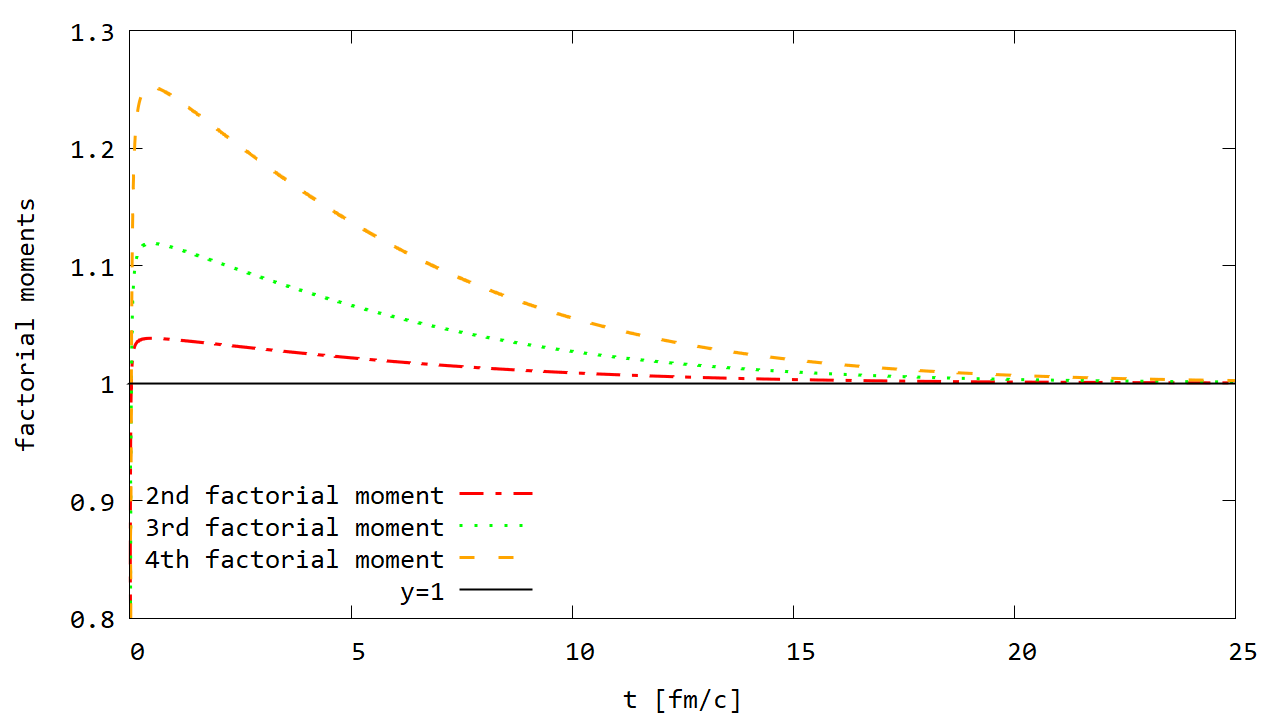
\includegraphics[width=1\textwidth, angle=0]{obrazky/fact_mom_T_165_jinak.png}
  	\caption[4. faktoriální moment pro různé teploty $T$]{Faktoriální momenty předělené svými rovnovážnými hodnotami pro teplotu $T = 165 ~\mathrm{MeV}$ pro 15 protonů a 10 pionů. \label{obr:F3}}
  \end{figure}
 
 \clearpage 
 \subsubsection{Postupná změna teploty}\label{sec:postupne}
 \indent
 
 
 Nyní necháme teplotu po úplné termalizaci faktoriálních momentů klesat podle Bjorkenova modelu z počáteční teploty $T_0 = 0.165 ~\mathrm{GeV}$ podle vztahu 
 
 \begin{equation}\label{eq:f26}
 T = T_0 \dfrac{t_0}{t}
 \end{equation}
 až na teplotu $T = 0.100 ~\mathrm{GeV}$.
 
 
 Čas $t_0$ je čas hadronizace pro teplotu $T = 0.165 ~\mathrm{GeV}$. Z Bjorkenovy závislosti teploty na čase je $t_0 = 6~\mathrm{fm/c}$.
 
  Zároveň s teplotou se mění i objem systému podle vztahu 
  
  \begin{equation}\label{eq:f38}
  V = V_0 \dfrac{t}{t_0},
  \end{equation}
  kde $V_0 = 125 ~\mathrm{fm^3}$.
  
  Pro numerické výpočty byly použity binomické počáteční podmínky s $N_0 = 0.005$.

 \begin{figure}[h!]
 	\centering	
 	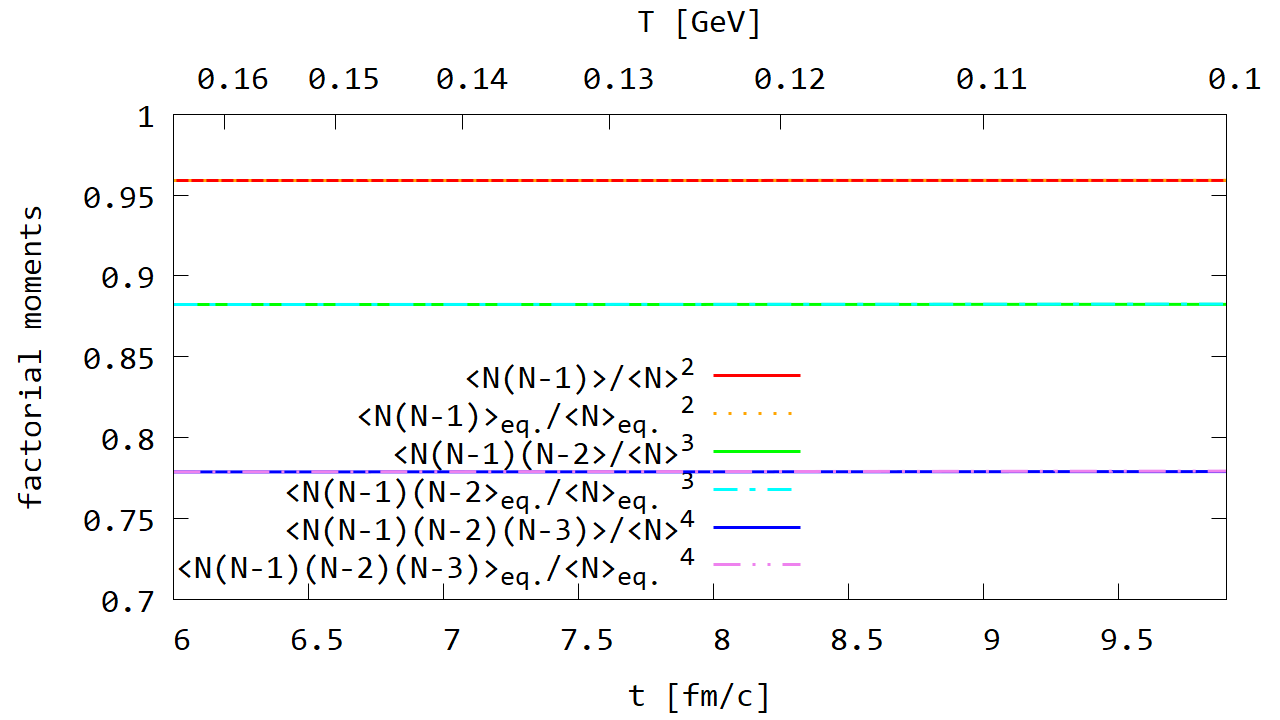
\includegraphics[width=0.8\textwidth, angle=0]{obrazky/fact_moments.png}
 	\caption[Normované faktoriální momenty pro postupnou změnu teploty ze 165 MeV na 100 MeV]{Normované faktoriální momenty pro postupnou změnu teploty ze 165 MeV na 100 MeV pro čas termalizace okolo $30 ~\mathrm{fm/c}$ a pro 15 protonů a 10 pionů. \label{obr:B10}}
 	
\end{comment}

 